\chapter[Determination of analysis parameters]{Determination of analysis parameters \label{chap:analysisparameters}}
% ----------------------------------------------------------------------------------------

The purpose of this chapter is to describe the tools included in the \diva software and that provide estimates of the analysis parameters: the correlation length $L$ and the signal-to-noise ratio $\snr$. The end of the chapter deals with the automatic quality control of data within the analysis.

\minitoc


%------------------------------------------------
\section{Determination of the correlation length}
%------------------------------------------------
\index{Correlation length}
The correlation length $L$ translates the distance over which a given data point influences its neighbourhood (Section~\ref{sec:parammeaning}). The method to evaluate $L$ is to fit the theoretical kernel of \eqref{divaformula2} (see Fig.~\ref{kernel1}) to the correlation between data assuming spatial isotropy and homogeneity in correlations.

\subsection{Illustration\label{sec:medseaex}}

This example employs salinity measurements in the Mediterranean Sea at a depth of 30~m in July, for the 1980-1990 period (Fig.~\ref{fig:diva_oi_09_10030dataval_mesh3}). The data set is built up by exploiting the SeaDataNet portal (\url{http://www.seadatanet.org}) and the World Ocean Database 2009 \citep[WOD09,][]{BOYER09} and contains 1061 data points. 

The regular grid for the analysis extends from 7$^{\circ}$W to 36$^{\circ}$E and from 30$^{\circ}$15'N to 45$^{\circ}$45'N, with a horizontal resolution of about 10~km. Measurements in the Black Sea and the Atlantic Ocean were removed in order to concentrate only on the Mediterranean Sea properties. The land-sea contours are created from the GEBCO bathymetry.

\begin{figure*}[h!]
\centering
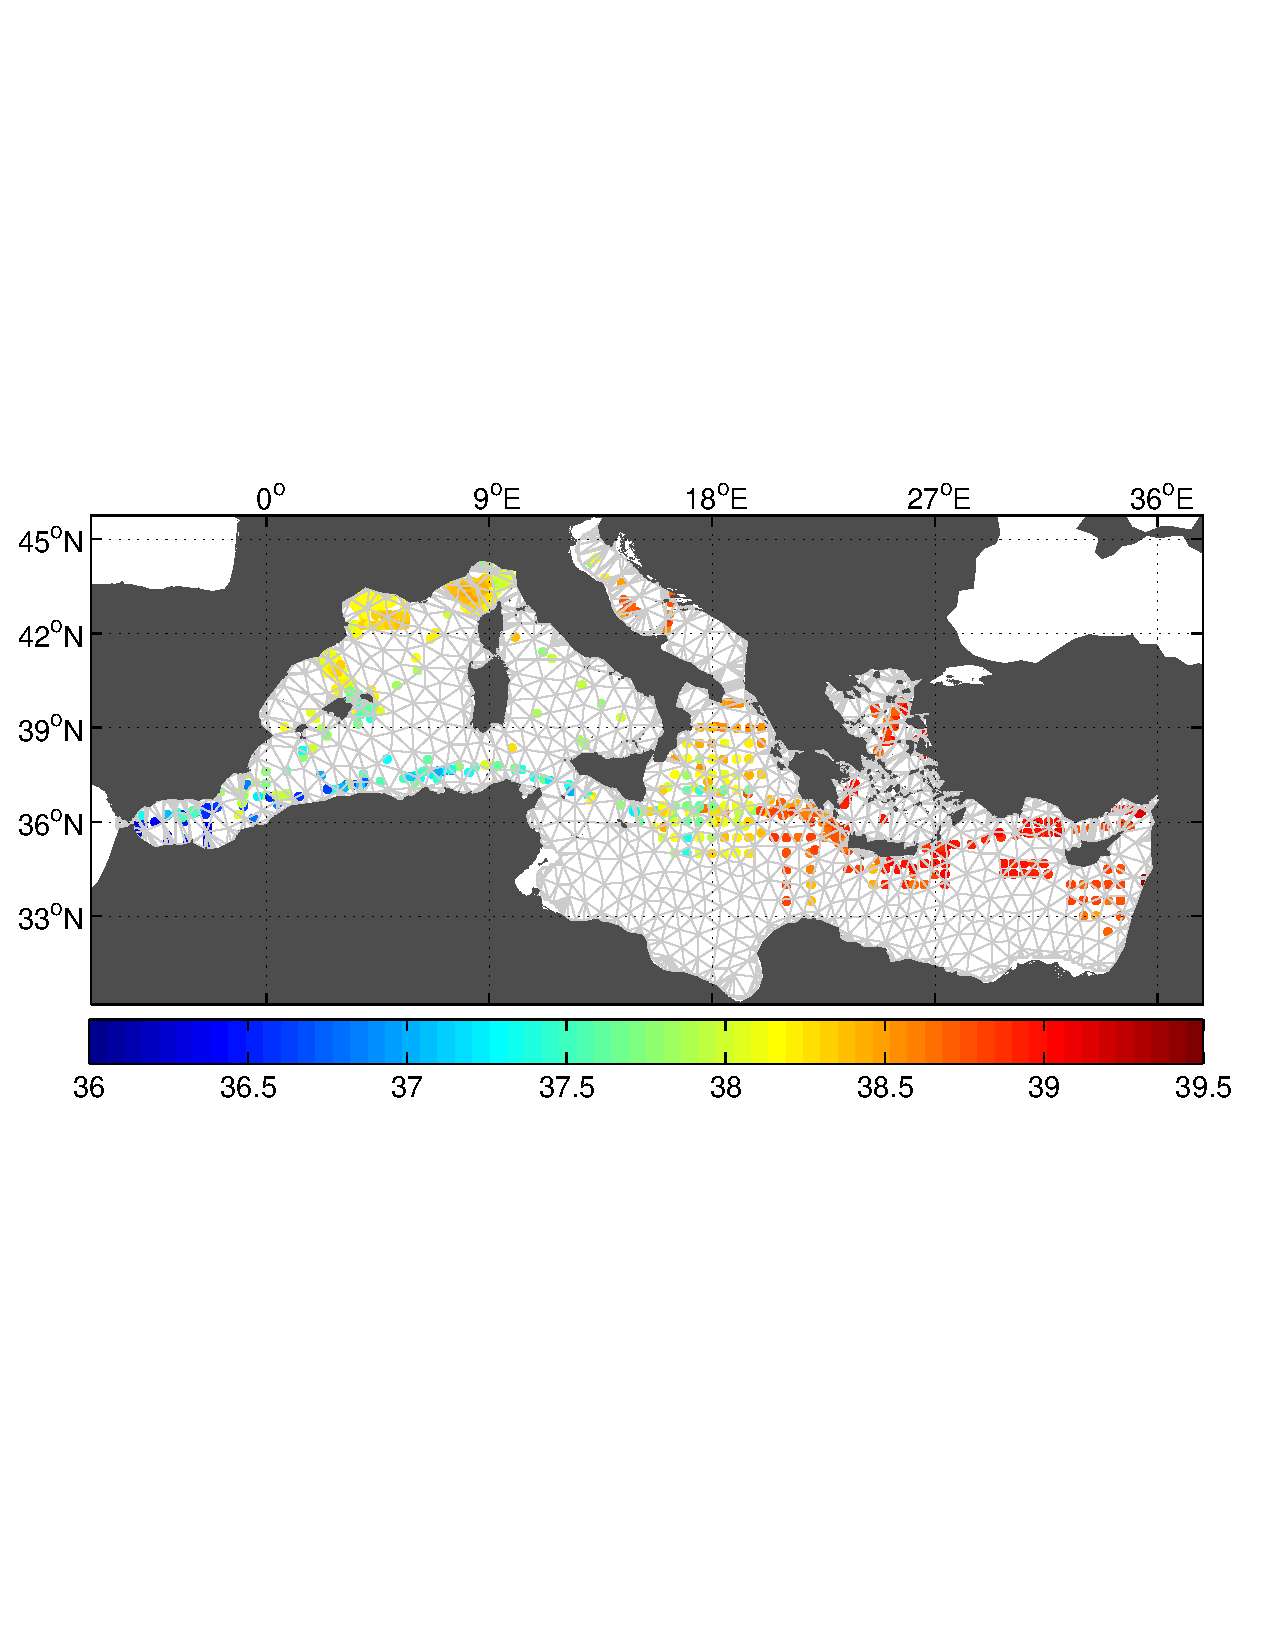
\includegraphics[width=.9\textwidth,bb=14 254 588 561]{diva_oi_09_10030dataval_mesh3}
\caption{Finite-element mesh and salinity measurements used for the application.\label{fig:diva_oi_09_10030dataval_mesh3}}
\end{figure*}

The fit yields the value $L=1.42^{\circ}$ ($\simeq$ 160~km).

\begin{figure}[h!]
\centering
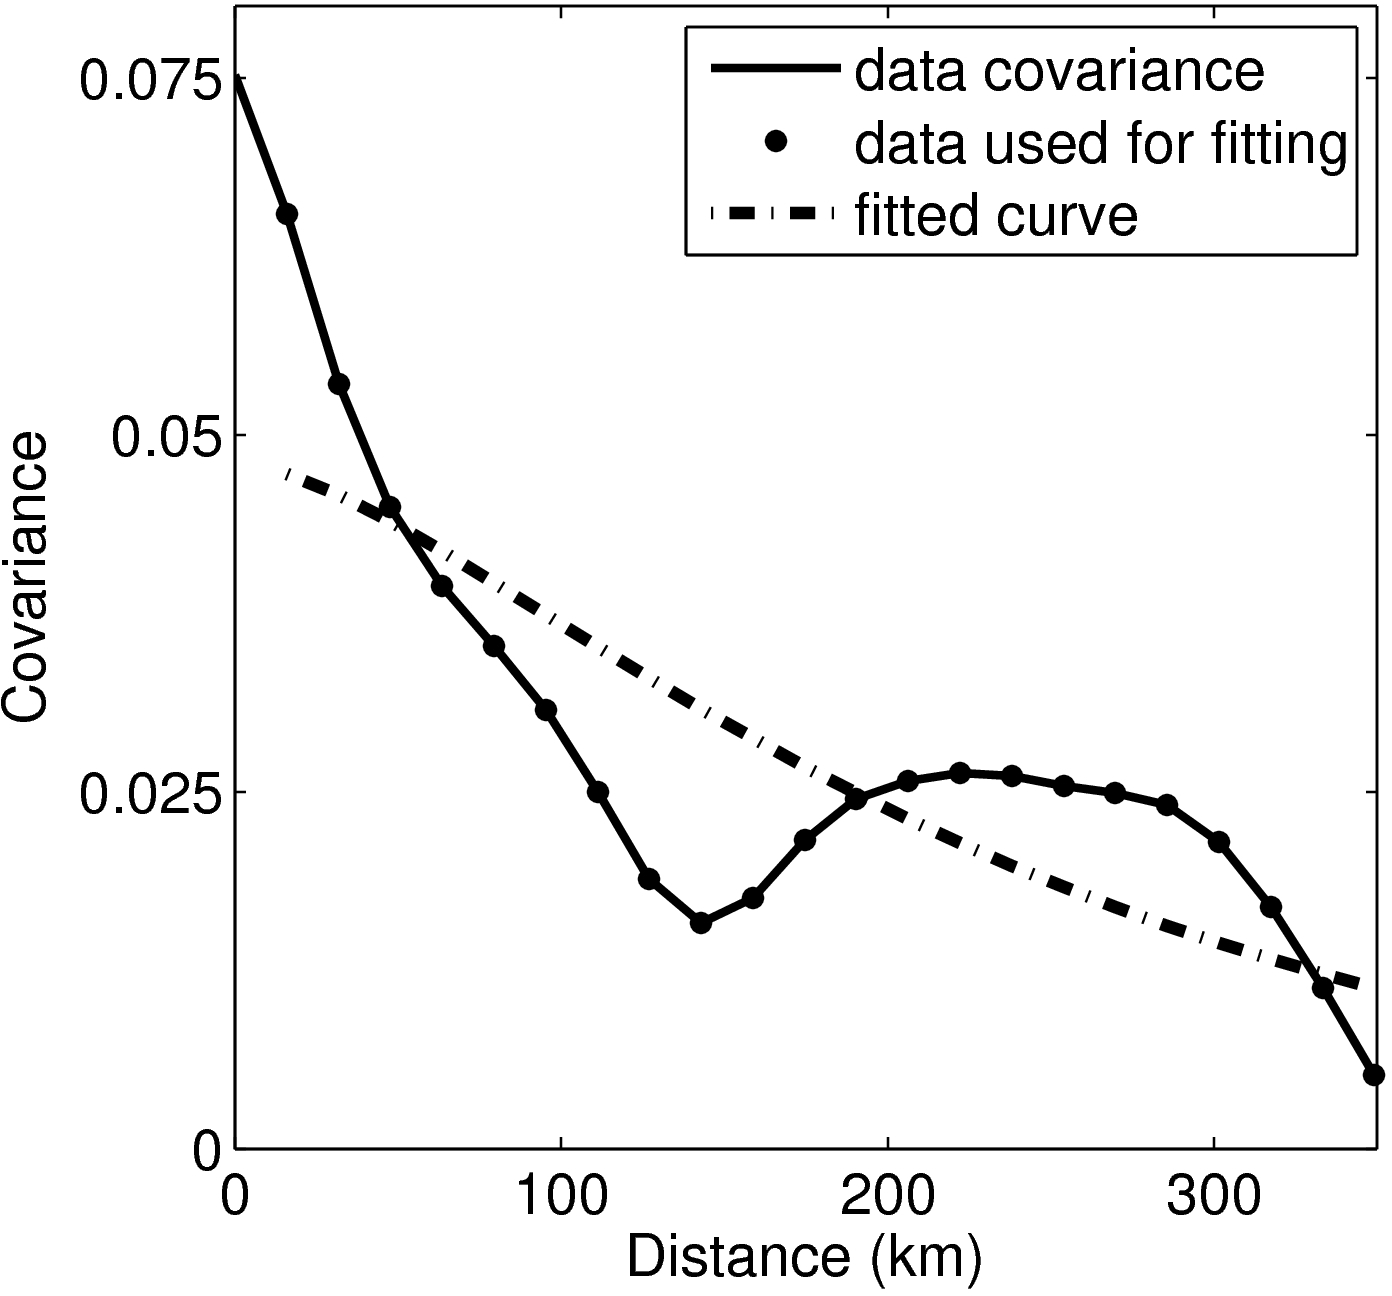
\includegraphics[width=.475\textwidth,bb=106 253 450 575]{Salinity_19502010_0707_10029e_fit}
\caption{Fit of the data correlation to the theoretical kernel (dashed line). \label{fig:Salinity_19502010_0707_10029e_fit}}
\end{figure}

\section{Determination of the signal-to-noise ratio}
%---------------------------------------------------

Once the correlation length is determined, the next step is to estimate the signal-to-noise ratio. 

\subsection{Generalities}
%------------------------

Let us consider the vector $\vect{d}$ containing the $N$ data anomalies. Objective analysis of $\vect{d}$ leads to analysed field with minimal expected error variance. The analysis $\varphi^a$ at any location $\vect{r}$ is given by
\begin{equation}
\varphi^a(\vect{r}) = \vect{c} \inv{(\matr{B}+\matr{R})} \matr{d}
\end{equation}
where $\vect{c}$ is a vector containing the background covariance between the point in which the analysis is to be performed and all data point locations. The optimal interpolation is based on the \textit{background covariance} matrix $\matr{B}$ and \textit{error covariance} matrix $\matr{R}$ of the data.
 
Let us call $\tilde{\vect{d}}$, the analysis vector at data points. The two vectors ${\vect{d}}$ and $\tilde{\vect{d}}$ can be related by the expression:

\begin{equation}
\tilde{\vect{d}}  =  \matr{A} \vect{d}
\end{equation}

where the matrix $\matr{A}$, used to perform the analysis at the data points, is calculated according to 

\begin{equation}
\matr{A}=\matr{B} \inv{(\matr{B}+\matr{R})}.
\end{equation}

The \textit{data-covariance} matrix is the statistical average $\mean{\quad}$ of data products:

\begin{equation}
\mean{\vect{d} \, \transp{\vect{d}}} = \matr{B}+\matr{R}, 
\label{eq:datavar}
\end{equation}
where $\transp{\,}$ it the transposed matrix or vector. For uncorrelated observational errors, error-covariance matrix $\matr{R}$ is diagonal, with a variance $\noise_i^2$ for point $i$, \textit{i.e.}

\[
\matr{R} = \mathrm{diag}(\noise_i^2)%\quad\textrm{or}\quad R_{ij}= \noise_i^2\delta_{ij}.
\]

In that case, we can show that the variance of expected misfit at point $i$ is
 
\begin{equation}
\mean{\left(d_i - \tilde{d}_i\right)^2} = \noise_i^2 (1 - A_{ii}).
\label{eq:epsilonmisfit}
\end{equation}

In practice covariance matrices are known only imperfectly: their structure is often considered to be
fixed, but with imperfectly known amplitude. In other words it is often assumed that

\begin{subeqnarray}
\matr{B}&=& \signal^2 \hat{\matr{B} },\label{eqcovA}\\
\quad \matr{R}&=& \noise^2 \hat{\matr{R} },\label{eqcovB}\\
\quad \frac{\transp{\vect{d}} \vect{d}}{N} &=& \signal^2 + \noise^2,\slabel{eqcovC}
\label{eqcov}
\end{subeqnarray}

where $\hat{ \quad } $ matrices are fixed and non-dimensional, while the field variance $\signal^2$ and the error variance
$\noise^2$ are imperfectly known, but their sum equal to the data variance (assuming that spatial averaging has a similar effect than statistical averaging, the ergodic hypothesis).

By definition of the average error- and field-variance, we have:

\begin{eqnarray}
\frac{1}{N} \sum_{i=1}^{N}\noise_{i}^{2} = \frac{1}{N} \trace{\matr{R}}=  \noise^2 \quad \Rightarrow \frac{1}{N} \trace{\hat{\matr{R}}}= 1 \label{eq:rcondition}\\
\frac{1}{N} \signal_{i}^{2} = \frac{1}{N} \trace{\matr{B}}=  \signal^2 \quad \Rightarrow \frac{1}{N} \trace{\hat{\matr{B}}}= 1
\end{eqnarray}

The unknown parameter that controls the analysis is the ratio of the signal and noise variances, called \textit{signal-to-noise ratio}:
\begin{equation}
\snr=\frac{\signal^2}{\noise^2},
\end{equation}
because matrix $\matr{A}$ depends only on $\lambda$:
\begin{equation}
\matr{A}(\snr)=\hat{\matr{B}} \inv{(\hat{\matr{B}}\, + \,\, \snr^{-1} \, \hat{\matr{R}})}.
\end{equation}


Dividing both sides of Eq. \eqref{eqcovC} by $\signal^{2}$ and  $\noise^{2}$, we also find that
\begin{eqnarray}
\signal^2 &=& \frac{\snr}{1 + \snr} \frac{ \transp{\vect{d}} \vect{d}}{N},\label{eq:signalsnr}\\
\noise^2 &=& \frac{1 }{ 1 + \snr} \frac{ \transp{\vect{d}} \vect{d} }{ N},\label{eq:noisesnr}
\end{eqnarray}
so that knowing $\snr$ we can calculate the signal and noise variances from the data values.

% ----------------------------------------------------------------------------------
\subsection{Ordinary Cross Validation (OCV)}
%-------------------------------------------

\index{Ordinary cross validation}
The objective is to optimize the parameter $\snr$ by searching for its value for which the analysis has a minimal error. For this reason, we need to find a proxy norm that we will be able to minimize. As the difference of the analysis with the true field is not available, we could try to work with the difference of the analysed field at the data points with respect to the original data field:

\begin{equation}
{\theta_i^2} = {(d_i - \tilde{d}_i)^2}.
\end{equation}

If we try to minimize this norm, we will get an infinite signal-to-noise ratio and a perfect data-analysis fit. This is because the analysis at the data point is directly influenced by the corresponding data. 

To avoid this inconvenience, the solution is to calculate the difference of the data value with respect to the analysed field in which the data under investigation was not taken into account. This is called the \textit{Ordinary Cross Validation} and is, with a practical trick, implemented in \command{divacv}. To make this estimate robust, the analysis has to be repeated over a large number of data points, increasing the computing cost, so that OCV is generally too expensive to perform unless a trick as in \command{divacv} can be used (there the analysis can be done without actually disregarding a data point but by correcting the difference as shown in the next section).

Variants of OCV take out several points at once to calculate error estimates and repeat the exercise several times to make estimates robust.  In \diva this options are available in \command{divacvrand}. A variant is \command{divacvclasses} in which all data from a given class (e.g. specific year) are set aside and the analysis compared to.


\subsection{Generalized Cross Validation (GCV)}
%----------------------------------------------

According to \citet{CRAVEN78}, modifying the error estimate as follows:

\begin{equation}
{\hat{\theta}_i^2} =  \frac{(d_i - \tilde{d}_i)^2}{(1 - A_{ii})^2}.
\label{eq:misfitestimate}
\end{equation}

allows one to keep the data during the analysis and will reduce the computing cost. In this formulation, the denominator penalizes more heavily data points in which the analysis is forced to be close the data and accounts therefore for the self-influence of the data point (which is absent in the case of pure cross-validation).

\subsubsection{Computation of $A_{ii}$}
% ---------------------------------------

When the matrix $\matr{A}$ is not explicitly calculated, $A_{ii}$ can be obtained by performing an analysis with a vector $\vect{e}_i=(0\,0\ldots\,0\,1\,0\ldots 0)$ (zero on all data locations, except at point $i$, where its value is one). This demands an analysis for every data point in which the estimator is constructed.  

The associated computational cost can be reduced by replacing $A_{ii}$ by the average value and assuming:
\begin{equation}
A_{ii} \simeq \frac{1}{N} \trace{\matr{A}}.
\label{eq:aiitrace}
\end{equation}

To avoid calculating all $A_{ii}$ and summing them up, we can use the following estimate \citep{GIRARD89}:
\begin{equation}
\frac{1}{N} \trace{\matr{A}} \simeq  \frac{ \transp{\vect{z}} \matr{A} \vect{z} }{\transp{\vect{z}} \vect{z} }
\label{eq:traceest}
\end{equation}
where $\vect{z}$ is a vector of random variables of zero mean. For robustness, the trace estimate can be repeated several times with different random vectors, averaging of the different estimates. The number of estimates is the parameter provided to the module \texttt{GCVFAC} of \diva.

Even if $\matr{A}$ is not available, $\matr{A} \vect{z}$ can be calculated easily by applying the analysis tool to a random vector and retrieve the analysis of this random vector on the data locations. Then the scalar product of the analysis of the random vector with the original random data provides the numerator of \eqref{eq:traceest} while the denominator is simply the squared norm of the random vector.

\subsubsection{Generalized cross validator}

In order to make the error estimator robust, we take the average over all data points and define the \textit{generalized cross validator} as 
\[
\Theta^{2}=\frac{1}{N}\sum_{i=1}^{N}\hat{\theta}_i^2.
\] 
Assuming temporarily $\noise_{i}^{2} = \noise^{2}$, hence having all misfits with the same weight, the generalized cross validator is obtained:

\begin{equation}
\Theta^2=\frac{\vnorm{\vect{d}-\tilde{\vect{d}}}^2}{N \left(1- \frac{1}{N}\trace{\matr{A}}\right)^2} 
        =\frac{\vnorm{(\matr{I}-\matr{A})\vect{d}}^2}{(1/N)\left(\trace{\matr{I}-\matr{A}}\right)^2}
\label{eq:gcv}
\end{equation}

The GCV consists in minimizing $\Theta^{2}$ by changing the signal-to-noise ratio $\snr$. $\Theta^2$ is a global estimate of the analysis error variance.

In view of \eqref{eq:epsilonmisfit} and \eqref{eq:gcv} the expected variance of the noise can also, by assuming a spatial average corresponds to a statistical expectation, be calculated as 
\begin{equation}
\epsilon^2 \simeq 
{\Theta^2  \left(1 - \frac{1}{N}\trace{\matr{A}}\right) }
\label{eq:noiseestimate}
\end{equation}


When the observational errors are uncorrelated but vary in space, we should replace the residual measure $r = \transp{(\vect{d}-\tilde{\vect{d}})} (\vect{d}-\tilde{\vect{d}}) $ by 

\begin{equation}
r = \transp{(\vect{d}-\tilde{\vect{d}})} \,\inv{ \hat{\matr{R}}} \,(\vect{d}-\tilde{\vect{d}})
\end{equation}
to take into account the relative noise level.

For a diagonal matrix, we can define weights $w_i$ such that

\begin{equation}
\epsilon^2_i = \frac{\epsilon^2}{w_i}= \frac{\sigma^2}{\lambda}\frac{1}{w_i}
\end{equation}

Defining the diagonal matrix $\matr{W} = \diag(w_i)$, the generalized cross validator then reads:

\begin{equation}
\Theta^2=\frac{ \transp{\left(\vect{d}-\tilde{\vect{d}}\right)} \matr{W} \left(\vect{d}-\tilde{\vect{d}}\right) }{ N \left(1 - \frac{1}{N}\trace{\matr{A}}\right)^2} 
\label{eq:gcvbis}
\end{equation}

where the weights should, according to \eqref{eq:rcondition} satisfy

\begin{equation}
\sum_i \frac{1 }{w_i} = N.
\label{eq:condition}
\end{equation}

The $\tilde{w}_i$ are the values provided as optional fourth column in \file{data.dat}.

\command{divacv} uses cross validation with complete calculation of $A_{ii}$, whereas \command{divagcv} uses the approximation $A_{ii} N=\trace{\matr{A}}$.

%------------------------------------------------------
\section{Quality control (QC) of data\label{secdivaqc}}
%------------------------------------------------------

Having defined the generalized cross validator, we look for a criterion that will allow the user to reject or accept a given data. Note that this QC is performed based on the analysis itself and shall be preceded by an a priori QC on the data (e.g., range of values, gradients, etc). 

\subsection{Quality criteria}
% ---------------------------

The first possibility is to compare the actual value of the misfit with the expected standard deviation $\mean{\left(d_i - \tilde{d}_i\right)^2}$, leading to the criterion:
\begin{eqnarray}
| d_i - \tilde{d}_i | > 3 \Delta_i^{(1)}\\
\textrm{with}  \qquad \Delta_i^{(1)} = \noise_i \sqrt{1-A_{ii}},\label{eq:qc1}
\end{eqnarray}
which is the most expensive version if $A_{ii}$ is not explicitly known and must be evaluated by analysis of vectors such as $\vect{e}_i=(0\,0\ldots\,0\,1\,0\ldots 0)$. 

If we replace $A_{ii}$ by its average $\frac{1}{N}\trace{\matr{A}}$, we have a second criterion based on:
\begin{equation}
\Delta_i^{(2)} = \noise_i \sqrt{ \left({1-\frac{1}{N} \trace{\matr{\matr{A}}}}\right)}. 
\label{eq:qc2}
\end{equation}
This version requires only a few analysis of a random vector if $\trace{\matr{A}}$ cannot be evaluated explicitly.


Finally, in case the noise is not calculated from $\Theta^2$, another estimate is then, according to \eqref{eq:noiseestimate}
\begin{equation}
\Delta_i^{(3)}= \frac{\noise_i}{\noise} { \left({1-\frac{1}{ N} \trace{\matr{A}}}\right)}\, \Theta,
\label{eq:qc3}
\end{equation}
which we can calculate directly from the RMS value of the misfit (or residual) and the generalized cross validator $\Theta$. This version can easily be used simultaneously with test \eqref{eq:qc2} using the results of the GCV.

 
\subsection{Normalized version}
% -----------------------------

Let us consider the scaled variable $s$ defined as
 
\begin{equation}
s_i = \frac{d_i - \tilde{d}_i}{\Delta_i}.
\end{equation}
 
Because we will look for outliers, instead of working with mean values and variances, more robust 
estimators are the median and $\mathrm{MAD}$ (\textit{median absolute deviation}).
 
A bias in the analysis is likely to exist if $S=\mathrm{median}(s_i)$ is not much smaller than one
(the typical values of $s$ should be of the order of one if the misfit estimate is correct on average).
 
Instead of calculating the standard deviation of $s$ we calculate 
the median absolute deviation  $\delta$ defined as

\begin{equation}
\delta = \mathrm{MAD}(s_i)=1.4826 \, \mathrm{median}| s_i-  S |
\end{equation}
where the factor 1.4826 is introduced such that for a normal distribution, the MAD is identical to the standard deviation.
 
Hence we can detect points qualified as outliers if they satisfy the inequality

\begin{equation}
|s_i-S | \ge 3 \delta.
\label{eq:qc4}
\end{equation}
 
This normalized version of quality control to some extent corrects for inaccurate estimation of the expected misfits $\Delta$.




\subsection{Implementation in \diva\label{sec:divagcv}}
%-------------------------------------------------------------------

\index{Signal-to-noise ratio} The overall signal-to-noise ratio $\snr$ is calculated as

\begin{equation}
\snr = \frac{\sigma^2 }{\epsilon^2}.
\end{equation}

The relative weights on the data are then defined as
\begin{equation}
\tilde{w}_i= \frac{\mu_i L^2}{4 \pi \lambda}.
\end{equation}

To be coherent with the total noise, we should in principle use relative weights (the optional fourth column for data in \diva) on the data that satisfy \eqref{eq:condition}.

Hence, defining $\bar{w}$ as
\begin{equation}
\frac{1}{\bar{w}} = \frac{1}{N} \sum_i \frac{1}{\tilde{w}_i},
\end{equation}
the weights $w_i=\tilde{w}_i/\bar{w}$ are relative weights coherent with the noise.

In this case, we can use \eqref{eq:gcvbis} for the estimator.

In practice, in \diva, the relative weights can be retrieved by $w_i=\mu_i/\bar{\mu}$, where
the average $\bar{\hphantom{\mu}}$ is a harmonic mean. The minimisation and the optimum for $\lambda$ are the same, even if the weights provided by the user do not satisfy the condition \eqref{eq:condition}. However the interpretation of $\Theta$, $\noise$ and $\sigma$ might be different.

Three scripts are available for the QC:
\begin{description}
\item[\command{divaqc}:] the most expensive version of QC, based on criterion \eqref{eq:qc1}.
\item[\command{divaqcbis}:] a quicker version, based on criterion \eqref{eq:qc2}.
\item[\command{divaqcter}:] based on the RMS value of the misfit and the generalized cross validator $\Theta$, according to criterion \eqref{eq:qc3}.
\end{description}


\subsubsection{\diva GCV practicals}

In \diva, the matrix $\matr{A}$ is not explicitly constructed, but the product $\matr{A} \vect{x}$ consists simply in the application of the analysis in data locations.

The value of $\trace{\matr{A}}$ can be evaluated and stored for subsequent quality control by \eqref{eq:qc2} and \eqref{eq:qc3}.
For quality control \eqref{eq:qc1}, $A_{ii}$ must be evaluated by an analysis of the pseudo-data vector $\vect{e}_i$ (zeros everywhere except unit value at point $i$). The analysis can benefit from the \textsf{LU} decomposition already performed for previous analysis.


